<<<<<<< HEAD:Course/FYS2140-Kvantefysikk.tex
% \RequirePackage{etoolbox}
% \RequirePackage{l3benchmark}
% \ExplSyntaxOn
% \AfterEndDocument { \benchmark_toc: }
% \use:n
%   {
%     \ExplSyntaxOff
%     \benchmark_tic:
%   }
  
=======
>>>>>>> parent of 85c40a3 (oblig 1):FYS2140-Kvantefysikk.tex
\documentclass[12pt]{report}
% \pdfcompresslevel=0
% \pdfobjcompresslevel=0
% \usepackage[timer=true]{regstats}
\usepackage{amsmath}
\usepackage[mathletters]{ucs}
\usepackage[utf8x]{inputenc}
\usepackage[margin=1.5in]{geometry}
\usepackage{enumerate}
\newtheorem{theorem}{Theorem}
\usepackage[dvipsnames]{xcolor}
\setlength{\parindent}{0cm}
% \usepackage{graphics}
\usepackage{graphicx} % Required for including images
\usepackage{subcaption}
\usepackage{bigintcalc}
\usepackage{pythonhighlight} %for pythonkode \begin{python}   \end{python}
\usepackage{appendix}
\usepackage{arydshln}
<<<<<<< HEAD:Course/FYS2140-Kvantefysikk.tex
% \usepackage{pgfplots}
% \pgfplotsset{compat/show suggested version=false}
% \usepackage{tikz-cd}
=======
\usepackage{physics}
\usepackage{tikz-cd}
>>>>>>> parent of 85c40a3 (oblig 1):FYS2140-Kvantefysikk.tex
\usepackage{booktabs} 
\usepackage{adjustbox}
\usepackage{mdframed}
\usepackage{relsize}
\usepackage{physics}
\usepackage[thinc]{esdiff}
\usepackage{fixltx2e}
\usepackage{esint}  %for lukket-linje-integral
\usepackage{xfrac} %for sfrac
\usepackage{hyperref} %for linker, må ha med hypersetup
\hypersetup{
    colorlinks = false,
    linkbordercolor = {white},
}
\usepackage[noabbrev, nameinlink]{cleveref} % to be loaded after hyperref
\usepackage{amssymb} %\mathbb{R} for reelle tall, \mathcal{B} for "matte"-font
\usepackage{listings} %for kode/lstlisting
\usepackage{verbatim}
\usepackage{graphicx,wrapfig,lipsum,caption} %for wrapping av bilder
\usepackage{mathtools} %for \abs{x}
\usepackage[norsk]{babel}
\definecolor{codegreen}{rgb}{0,0.6,0}
\definecolor{codegray}{rgb}{0.5,0.5,0.5}
\definecolor{codepurple}{rgb}{0.58,0,0.82}
\definecolor{backcolour}{rgb}{0.95,0.95,0.92}

\lstdefinestyle{mystyle}{
    backgroundcolor=\color{backcolour},   
    commentstyle=\color{codegreen},
    keywordstyle=\color{magenta},
    numberstyle=\tiny\color{codegray},
    stringstyle=\color{codepurple},
    basicstyle=\ttfamily\footnotesize,
    breakatwhitespace=false,         
    breaklines=true,                 
    captionpos=b,                    
    keepspaces=true,                 
    numbers=left,                    
    numbersep=5pt,                  
    showspaces=false,                
    showstringspaces=false,
    showtabs=false,                  
    tabsize=2
}

\lstset{style=mystyle}
\author{Oskar Idland}
\title{FYS2140 - Kvantefysikk}
\date{}
<<<<<<< HEAD:Course/FYS2140-Kvantefysikk.tex
% \includeonly{17 Forelesnings Notater} 
=======

>>>>>>> parent of 85c40a3 (oblig 1):FYS2140-Kvantefysikk.tex
\begin{document}
\maketitle
\newpage
\tableofcontents
\newpage
\part{Historisk Utvikling}
\chapter{Bruddet med Klassisk Fysikk}
\section{Hva er Kvantemekanikk?} 
Kvantemekanikk forsøker å beskrive fysiske systemer på kvante nivå. Her står Schrödinger's likning sentralt. 

\subsection{Energikvantisering}
Energi i Kvantemekanikken er ikke en kontinuerlig størrelse. Den har diskrée verdier. Dette kalles energikvantisering. Dette gjelder både fotoner og elektroner. 

\subsection{Bølge-Partikkel-dualitet}
Vi vet ikke helt hva er partikkel er, men det vi vet er at de har egenskaper som minner om partikler og bølger. Dette kalles bølge-partikkel-dualiteten. Vi kan skyte ut fotoner i små energi pakker eller kvanter hvor de vil oppføre seg som partikler, men som en ser i dobbelspalteeksperimentet kan de likevel oppføre seg som bølger på samme tid. Da trenger vi Schrödinger's bølgeligning.

\subsection{Egentilstand og superposisjon}
En partikkel med kvantisert energien $ ϵ_{n} $ befinner seg i en tilstand som er beskrevet av bølgefunksjonen $ ψ_{n} $. Dette kalles en energi-egentilstand. En partikkel kan være i flere energi-egentilstander samtidig. Dette kalles superposisjon. Vi kan tenke på Schrödinger's katt som en partikkel som er i en superposisjon av to energi-egentilstander, død og levende. Da får vi følgende:
\begin{equation}
ψ = c_{\text{død}} ⋅ ψ_{\text{død}} + c_{\text{levende}} ⋅ ψ_{\text{levende}}
\end{equation}
Hvis vi måler tilstanden til katten vil vi få én av de to tilstandene. Enten død eller levende. Da ender vi opp i det som kalles \textit{egentilstand} fra bølgefunksjonen/superposisjon. Sannsynligheten for at katten er død er da $ \left\vert c_{\text{død}} \right\vert ^{2} $ og Sannsynligheten for at katten er levende er $ \left\vert c_{\text{levende}} \right\vert ^{2} $. Det eneste Kvantemekanikken kan fortelle oss er sannsynligheten for at katten er i en tilstand, ikke om den er i den tilstanden eller ikke, før vi måler det. 

\subsection{Heisenberg's uskarphetsrelasjon}
I klassisk mekanikk er foreksempel posisjon $ \mathbf{x} $ og bevegelsesmengde $ \mathbf{p} $ uavhengig størrelser. I Kvantemekanikken impliserer via Heisenberg's uskarphetsrelasjon at en ikke kan observerer begge til en vilkårlig presisjon. Dette uttrykkes via følgende formel
\begin{equation}
Δ \mathbf{p} Δ\mathbf{x} \geq \frac{ℏ}{2}
\end{equation}
hvor $ Δ\mathbf{x} $ er usikkerheten i posisjon og $ Δ\mathbf{p} 
$ er usikkerheten i bevegelsesmengde. Dette er bare en merkbart på atomært nivå, men gjelder teknisk sett alltid. 

\subsection{Paulis eksklusjonsprinsipp}
To fermioner (f.eks elektroner, protoner, kvarker og nøytrinoer) akn ikke befinne seg i samme tilstand (dvs. samme energi samme sted). Dette ser vi i atomer hvor elektronene fyller opp skall slik at nye elektroner må fylle opp et nytt skall. 



\section{Enheter i Kvantefysikk}
\subsection{Lengde}
For å unngå ekstremt små eller store tall bruker vi litt smarte enheter. Kvantefysikken operer på størrelser fra $ 10^{-8} $ til $ 10^{18} $m. Nanometer (nm) er $ 10^{-9} $m, femtometer (fm) er $ 10^{-15} $m og ångstrøm (Å) er $ 10^{-10} $m / $ 0.1 $nm.

\subsection{Energi}
For energi brukes til vanlig Joule, men energien i kvantemekanikken er så liten som $ 10^{-19} $J. Da bruker vi eV (elektronvolt) som er $ 1.602 \cdot 10^{-19} $C. Dette kommer fra at 1J er likt med 1C $\cdot$ 1V. Da er 1 eV den kinetiske energien et elektron får når den akselereres gjennom en potensialdifferensen på 1V. 

\subsection{Masse}

Istedet for å bruke kg for å måle masse kan vi heller bruke MeV/c$^{2}$. Dette kommer fra likningen $ E = mc^{2} $. Ser vi på hvileenergien til med enheten eV får vi 
\begin{equation}
E_{0}^{\text{elektron}} = m_{e} c^{2} = 5.11 \cdot 10^{5} \text{eV}
\end{equation}
Løser vi dette for massen $ m_{e} $ får vi
\begin{equation}
m_e = E_{0}^{\text{elektron}} / c^{2} = 0.511\ \text{MeV}/c^{2}
\end{equation}

\subsection{Andre Konstanter}
\textbf{Placks konstant}
\begin{equation}
h = 6.626 ⋅  10^{-34} \text{ Js} = 4.135 ⋅ 10^{-15} \text{  eVs}
\end{equation}
\begin{equation}
ℏ = \frac{h}{2 \pi} = 1.055 ⋅ 10^{-34} \text{Js} = 6.582 ⋅ 10^{-16} \text{eVs} 
\end{equation}
\begin{equation}
hc = 1240 \text{ eV nm} (\text{MeV fm})
\end{equation}
\begin{equation}
ℏc = 197.3 \text{ eV nm} (\text{MeV fm})
\end{equation}
Noen ganger kan det lønne seg å gange en brøk med $ c $ oppe og nede for å få inn konstanten $ ℏc $. Utrykket under hadde medført veldig små størrelser ($ 10^{-34} $ og $ 10^{-31} $) og dermed ville det blitt vanskelig å regne med. 
\begin{equation}
\frac{h}{m_e c} = \frac{hc}{m_e c^{2}} = \frac{1240 \text{eV nm}}{0.511 ⋅ 10^{6}} ≈ 0.002 nm
\end{equation}
\subsection{Coulomb-potensialet}
\begin{equation}
V(r) = \frac{e^{2}}{4 \pi \epsilon_{0} r} = \frac{k_e e^{2}}{2}, \qquad k_e e^{2} = 1.44 \text{eV nm}
\end{equation}
\subsection{Nyttige Tabeller}

\begin{figure}[ht!]
  \centering
  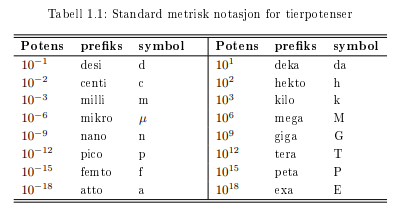
\includegraphics[scale = 1]{Figures/Metric power notation .png}
  \caption{}
  \label{fig: Metric power notation}
\end{figure}

\begin{figure}[ht!]
  \centering
  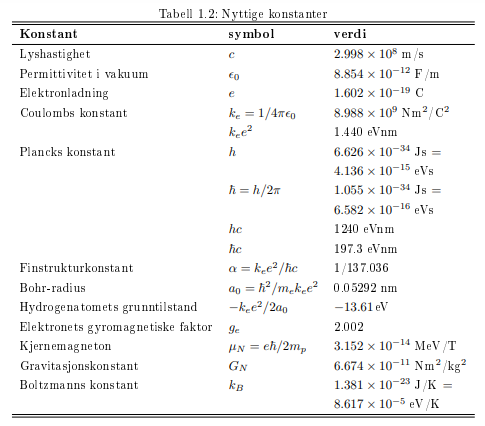
\includegraphics[scale = 1]{Figures/Constants table.png}
  \caption{}
  \label{fig: Constants table}
\end{figure}

\begin{figure}[ht!]
  \centering
  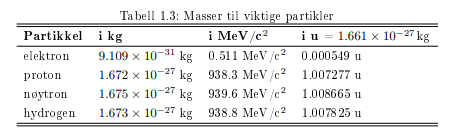
\includegraphics[scale = 1]{Figures/Masser til viktige partikler.png}
  \caption{}
  \label{fig: Masser til viktige partikler}
\end{figure}

\begin{figure}[ht!]
  \centering
  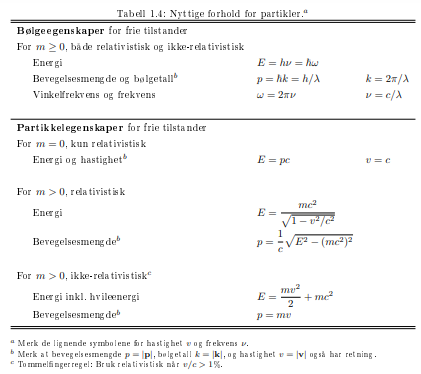
\includegraphics[scale = 1]{Figures/Nyttige forhold for partikler.png}
  \caption{}
  \label{fig: Nyttige forhold for partikler}
\end{figure}

\newpage

\section{Planck's Kvantiseringshypotese}
Kvantisering betyr i kvantefysikken at en fysisk størrelse bare antar diskrete verdier. Eksempler på dette er elektrisk ladning, hvor fri ladning er et heltallig $ \mathbb{N} $ multiplum av antall frie elektroner. Energi kan også kvantifiseres og var definerende for bruddet med klassisk fysikk. Klassisk fysikk klarer ikke å forklare frekvensfordelingen til elektromagnetisk stråling fra et legeme ved en gitt temperatur. Dette kan være sola eller en vanlig stekeplate. 
\subsubsection*{Definisjoner}
\begin{itemize}
    \item \textbf{Termisk stråling}: Elektromagnetisk stråling sendt ut av et materiale ved en temperatur $ T $. Alle legemer emitterer og absorber denne strålingen
    \item Ved en gitt temperatur $ T $ er vi interessert i å finne fordelingen av emittert stråling som funksjon av den elektromagnetiske strålingen sin frekvens $ ν $ eller bølgelengde $ λ $. Forholdet mellom frekvens $ ν $ og bølgelengde $ λ $ er gitt ved
    \begin{equation}
    ν = \frac{c}{λ}
    \end{equation}
    
    \item \textbf{Frekvensfordeling}
    \begin{equation}
    M_{ν}(T)
    \end{equation}
    Kalles spektralfordelingen eller fordelingsfunksjonen for frekvensspekteret beskriver mengden utstrålt energi fra en gjenstand ved temperatur $ T $ per areal per tid per frekvensenhet. 
    
    \item Integrert over alle frekvenser 
    \begin{equation}
    M(T) = \int_{0}^{\infty} M_{ν}(T) \ dν
    \end{equation}
    får vi totalt utstrålt energi per sekund per areal ved en gitt temperatur $ T $. Enhetene bli følgende: M(T) = $ J / m^{2}s = W / m^{2} $. Dette kalles radians. 
    
    \begin{figure}[h!]
        \centering
        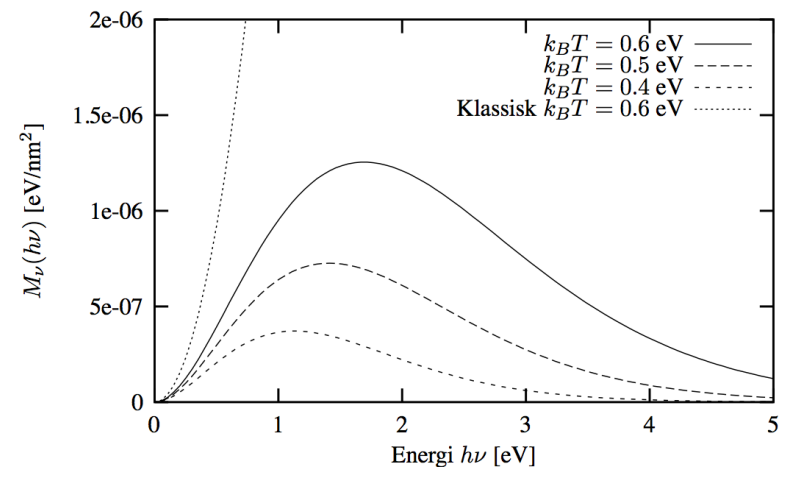
\includegraphics[scale = .5]{Figures/Frekvensfordeling kvantiserinspostulat.png}
        \caption{Frekvensfordelingen fra Planck's kvantiseringspostulat. Merk den klassiske kurven som øker alt for mye ikke matcher observert frekvens}
        \label{fig: Frekvensfordeling kvantiserinspostulat}
    \end{figure}
    
    \item \textbf{Vår utfordring er å finne frem til en forklaring for den eksperimentell formen til} $M_{ν}(T)$
\end{itemize}

Den klassiske versjonen å se på dette var via et sort legeme som er tenkt til å ikke reflektere noe av strålingen den mottar, alt blir absorbert. Dette ble det eksperimentert og resultatet ser man i figur \ref{fig: Frekvensfordeling kvantiserinspostulat}. 
Basert på måledata kom en fram til at radiansen til et sort legeme kan skrives som 
\begin{equation}
M(T) = σT^{4}
\end{equation}
hvor $σ$ er en konstant. Dette kalles Stefan-Boltzmanns lov. Wiens forskyvningslov beskriver sammenhengen mellom temperaturer og bølgelengden $λ_{\text{max}}$. 
\begin{equation}
λ_{\text{max}}T = 2.897 ⋅ 10^{-3} \text{ mK}
\end{equation}
Nå skal vi se hva som skjer når vi bruker resultatene fra klassisk fysikk. 
\begin{equation}
M_{ν}(T) = \frac{2 π ν^{2}}{c^{2}} \left< E \right>
\end{equation}
hvor $\left< E \right>$ er gjennomsnitsenergien per svingemode til det elektromagnetiske feltet i hulrommet til det sorte legeme. 
\begin{equation}
\left< E \right> = k_{B}T
\end{equation}
hvor $k_{B}$ er Boltzmanns konstant. For å finne radiansen setter vi inn utrykket for $\left< E \right>$ og integrerer. 
\begin{equation}
M(T) = \int_{0}^{∞} \frac{2 π v^{2}}{c^{2}} k_{B}T \ \mathrm{d}ν
\end{equation}
Dette er lett å se at energien går mot uendelig og matcher ikke med de eksperimentelle resultatene. En formel som matcher bedre kan ikke divergere. Feilen er at $\left< E \right>$ er ikke stemmer. Hvis en ser på strålingen som et stort antall kvantiserte enheter med energi $ϵ_{n}$
\begin{equation}
ϵ_{n} = nhν
\end{equation}
der $h$ er Planck's konstant og $n$ er et heltall. Planck utledet et alternativt utrykk for $\left< E \right>$. 
\begin{equation}
\left< E \right> = \frac{hν}{e^{hν/k_{B}T} - 1}
\end{equation}
Som gir
\begin{equation}
M_{ν}(T) = \frac{2 π ν^{2}}{c^{2}} \frac{hν}{e^{hν/k_{B}T} - 1}
\end{equation}
Som samsvarer med eksperiment. Viktig å få med seg er at $\left< E \right> → k_{B}T$ når $T → ∞$ eller $λ → \infty$ aka $ν → 0$ som er hvor klassisk mekanikk er gyldig.
For å få litt mer elegante utrykk å unngå store eller små tall ganger vi inn $h$. 
\begin{equation}
M_{ν}(T) = \frac{2π}{h^{2}c^{2}} \frac{(hν)^{3}}{e^{h ν/k_{B}T} - 1}
\end{equation}

Vi setter in $x = hν$
\begin{equation}
M_{x}(T) = \frac{2π}{h^{2}c^{2}} \frac{x^{3}}{e^{x/k_{B}T} - 1}
\end{equation}
Vi vet at $hc = 1240 $eV nm 
\begin{equation}
M_{x}(T) = \frac{2π}{1240^{2}} \frac{x^{3}}{e^{x/k_{B}T} - 1}
\end{equation}

Hvor $M_{x}$ har enheter eV / nm$^{2}$. For å utlede Stefan-Boltzmanns lov via Planck's utrykk bruker vi den originale formelen og setter in x vi fant tidligere. 
\begin{equation}
M(T) = \int_{0}^{∞} M_{ν}(T) \ \mathrm{d}ν = \int_{0}^{∞} \frac{2πν^{2}}{c^{2}} \frac{hν}{e^{hν / k_{B}T} - 1} \ \mathrm{d}ν
\end{equation} 

\begin{equation}
M(T) = \frac{2πk^{4}_{B}}{c^{2}h^{3}}T^{4} \underbrace{\int_{0}^{∞} \frac{x^{3}}{e^{x} - 1} \ \mathrm{d}x}_{\frac{π^{4}}{15}}
\end{equation}

\begin{equation}
M(T) = σT^{4}, \quad σ = \frac{2π^{5}k^{4}_{B}}{15c^{2}h^{3}} = 5.676 ⋅ 10^{-8} \frac{\text{W}}{\text{m}^{2} \text{K}^{4}}
\end{equation}

Den viktigste forskjellen var at Planck regnet ut den midlere verdien $\left< E \right>$ med diskrete verdier for energi og ikke kontinuerlige verdier. Han hadde dataen foran seg og prøvde å finne en modell som passet. 

\subsubsection*{Plank's Hypotese}
Enhver fysisk størrelse som utviser enkle harmoniske svingninger har energier som tilfredsstille
\begin{equation}
E_n(ν) = nhν, \qquad n = 1, 2, 3, \dots
\end{equation}

hvor $ν$ er frekvensen til svingningene og $h$ er en universell konstant. 

Kvantefysikken gjelder alltid, men klassisk fysikk kan brukes når energiskalaen er stor nok ettersom det ikke er merkbart. 

\subsection{Utledning av Wiens Forskyvningslov}
\include{Kvantemekanikkens matematiske spraak}
\include{Andvendelser}
<<<<<<< HEAD:Course/FYS2140-Kvantefysikk.tex
\part{Forelesning Notater}

\chapter{Lysets Partikkelegenskaper}
=======
\part{Lecture Notes}
>>>>>>> parent of 85c40a3 (oblig 1):FYS2140-Kvantefysikk.tex
\chapter{02 Forelesnings Notater}
\section{Definisjoner}
\subsection{Sort legeme}    
Et sort legemet absorberer alt av stråling og vil ved lave temperaturer se helt sort ut. Ved høyere temperaturer vil den gløde. 

\subsection{Frekvensfordeling $M_{ν}(T)$}
Funksjonen som viser fordelingen av forskjellige temperaturer i et sort legeme. 

\subsection{Radians $M(T)$}
Total mengde energi et sort legemet stråler ut. 
\begin{equation}
M(T) = \int_{0}^{∞} M_{ν}(T) \ \mathrm{d}ν
\end{equation}

\subsection{Stående bølge}
En stående bølge er en bølge som ikke beveger seg. 

\chapter{03 Forelesning Notater}
\section{Sentrale Kunnskaper}
\begin{itemize}
    \item Beskrive den fotoelektriske effekten og 
    \item Hvordan Einsteins teori forklarer de tre ekps. observasjonene. Forstå hva det betyr at et materialet har arbeidsfunksjon $w_0$. Håndtere og beregne $K_{\text{max}} = hν - w_0$
    \item Beskrive hvordan Röntgen-stråling-eksp. støtter Einsteins teori.
\end{itemize}
\section{Fotoelektrisk Effekt}


\begin{figure}[h!]
  \centering
  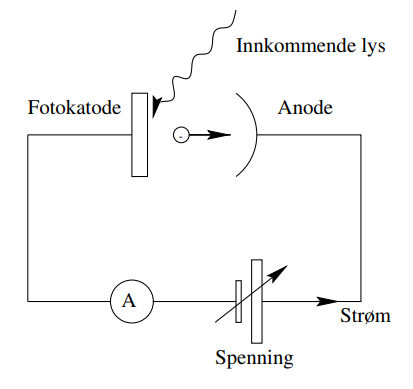
\includegraphics[scale = .5]{Figures/Fotoeletkrisk effekt oppsett.png}
  \caption{Oppsett av den fotoelektriske effekten}
  \label{fig: Fotoelektrisk effekt oppsett}
\end{figure}
Spenningen $V$ fra Anoden til Fotokatoden skaper et elektrisk felt fra Anoden til Fotokatoden. Her går det ikke noe strøm. Hvis vi sender elektromagnetisk stråling på Fotokatoden får vi en fotostrøm strøm gjennom kretsen. Dette må bety at strålingen frigjør elektroner i materialet.

Intensiteten til lyset definers som $I = \frac{E}{As}$ hvor $E$ er energi, $s$ er tid og $A$ er areal. Intensitet måles i $W / m^{2}$

Den kinetiske energien $K$ til et elektron er definert ved overflaten til materialet til Fotokatoden. 

Det elektriske feltet vil akselererer elektronene som fører til en økning i kinetisk energi gitt ved 
\[
K + eV. 
\]
Illustrert i figur \ref{fig: Fotoelektrisk effekt oppsett}, har vi en positiv spenning ved Anoden. Hvis vi snur dette til en negativ spenning $-V$. Da vil elektronene ha en kinetisk energi $K_{\text{overflate}}$, som motvirkes av det elektriske feltet. Elektronene vil da gå tilbake til materialet. Hvis den kinetiske energien er høy nok kan elektronene nå frem til Anoden i andre enden. Da blir den kinetiske energien $K = K_{\text{overflate}} - \left\vert eV \right\vert $. Da må naturligvis $K_{\text{overlfate}} \ge  eV$. 

Dette fenomenet ble avdekket tre observasjoner. 

\subsection{Observasjon 1}
For å undersøke strømmen som funksjon av spenningen setter vi en konstant intensitet og frekvens på lyset. Når vi minker spenningen vil strømmen også minke ettersom elektronene krever mer kinetisk energi for å nå Anoden. Til slutt vil strømmen ta fullstendig slutt når vi setter på en spenning $-V_0$. Ved denne spenningen er $K < \left\vert eV_0 \right\vert $. Vi setter da $K_{\text{maks}} = \left\vert eV_0 \right\vert $. Strømmen med dette oppsette er notert ved $I_1$ sett i figur \ref{fig: Fotoelektrisk resultat}

\begin{figure}[h!]
  \centering
  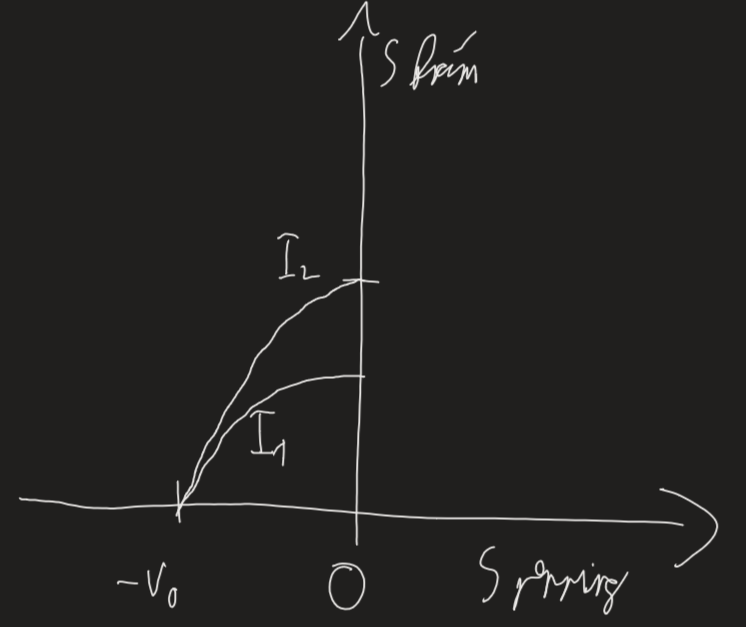
\includegraphics[scale = .4]{Figures/Fotoelektrisk resultat.png}
  \caption{Eksperimentelle resultater av fotoelektrisk effekt}
  \label{fig: Fotoelektrisk resultat}
\end{figure}


Nå kommer det som kræsjer med klassisk fysikk. Hvis vi øker intensiteten på strålingen forventer vi at elektronene får høyere kinetisk energi, og flere elektroner blir en del av fotostrømmen. Det stemmer at en får mer strøm $I_2$, men strømmen stopper ved samme spenning $-V_0$ som sett i figur \ref{fig: Fotoelektrisk resultat}. 

\subsection{Observasjon 2}
Neste forsøk som sett i figur \ref{fig: Fotoelektrisk resultat 2} valgte man å holde intensitet konstant og varierer spenningen $ν$. Da ser man at max kinetisk energi øker lineært med frekvensen på lyset. $K_{\text{max}}$ går mot null når frekvensen går mot $ν_0 > 0$. Frekvensen dikterer hva som er den maksimale kinetiske energien til elektronene, og dermed størrelsen på spenningen $V_0$ som sett i figur \ref{fig: fotoelektrisk resultat 2.1}.
\begin{figure}[h!]
  \centering
  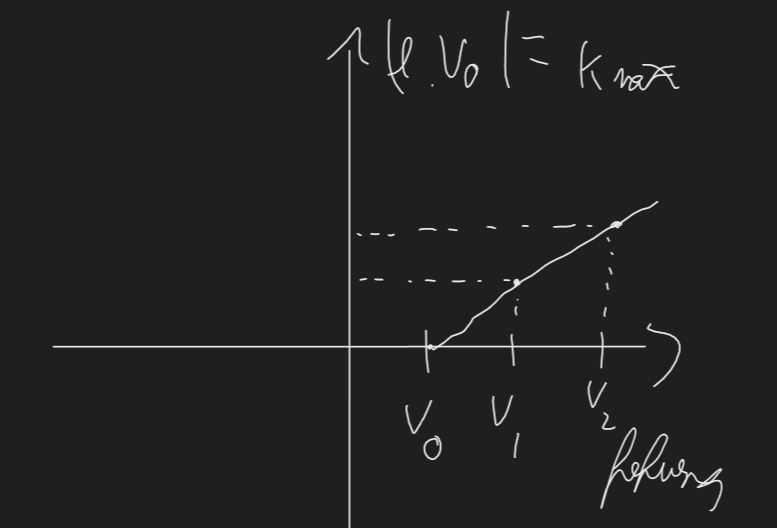
\includegraphics[scale = .4]{Figures/Fotoelektrisk resultat 2.png}
  \caption{Eksperimentelle resultater av fotoelektrisk effekt med varierende frekvens $ν$}
  \label{fig: Fotoelektrisk resultat 2}
\end{figure}

\begin{figure}[h!]
    \centering
    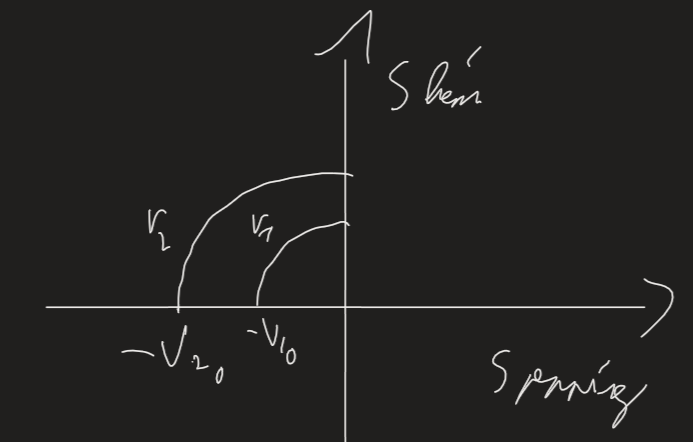
\includegraphics[scale = .4]{Figures/fotoelektrisk resultat 2.1.png}
    \caption{Strøm som en funksjon av spenning}
    \label{fig: fotoelektrisk resultat 2.1}
  \end{figure}


\subsection{Observasjon 3}
En la merke til at fotostrømmen skjer nesten øyeblikkelig. Det betyr at det elektronene ikke krever mye tid for å få en kinetisk energi $K = \left\vert eV_0 \right\vert $. Dette er uavhengig av intensiteten på strålingen.

\subsubsection{Oppsummert}
  1a. Det eksisterer en stoppepotensial $V_0$, og ingen elektroner har $K \ge  \left\vert eV_0 \right\vert $. 
  
  1b. $K_{\text{maks}} = \left\vert e V_0 \right\vert $ uavhengig av intensiteten på strålingen.
  
  2a. $K_{\text{maks}}$ øker lineært med frekvensen på strålingen.
  
  2b. $K_{\text{maks}}$ går mot null når frekvensen går mot $ν_0 > 0$
  
  3. Fotostrømmen skjer nesten øyeblikkelig.

\subsubsection{Einsteins Forklaring}
Einstein så på lyset som små energi pakker i stedet for et kontinuerlig bølgefelt. Hvert foton vil da ha en energi $E = hν$. Fotonene vil frigjøre elektronene i materialet. Dette vil da gi elektronene en energi $E = hν$, som kan være nok til å komme på utsiden av materialet. Det krever litt energi så elektronet vil ha en kinetisk energi $K = hν - ω$, der $ω$ er energien tapt på vei til overflaten. Da vil $K_{\text{maks}} = hν - ω_0$ ettersom $ω_0$ er den minste energien som kreves for å løsrive det svakest bunnende elektronet. $ω_0$ er arbeidsfunksjonen. 

Dette er i et ideelt tilfelle hvor elektronene ikke kolliderer med hverandre eller går i andre retninger enn rett mot Anoden. Det viktigste å få med seg er hvordan Einstein forklarer at $K_{\text{maks}}$ er uavhengig av intensiteten på strålingen, bare frekvensen. 


\section{Röntgen-Stråling}

\begin{figure}[h!]
    \centering
    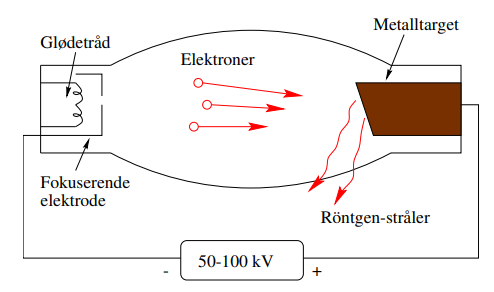
\includegraphics[scale = .5]{Figures/Rontgenstraaling oppsett.png}
    \caption{Oppsett av röntgenstråling eksperimentet}
    \label{fig: Rontgenstraaling oppsett}
\end{figure}

\begin{figure}[h!]
  \centering
  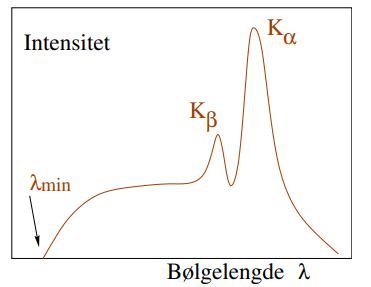
\includegraphics[scale = .5]{Figures/Rontgenstraaling intensitetfordeling.png}
  \caption{Intensitet fordeling ved Röntgenstråling}
  \label{fig: Intensitets fordeling Rontgenstraaling}
\end{figure}

Dette er det motsatte av fotoelektrisk effekt. Her skytes elektroner på et materialet som skyter ut fotoner. Den maksimale energien et utstrålt foton kan ha er gitt ved 
\[
E_{\text{maks}} = \frac{hc}{\lambda} = hν
\]

  
\chapter{04 Forelesnings Notater}
\section{Compton-Spredning}
\subsubsection{Sentrale kunnskaper}
\begin{itemize}
    \item Beskrive de fysiske modellene
    \item Vite at fotoner har bevegelsesmengde
    \item fotoner kolliderer med frie elektroner, eller med tunge atomer 
    \item Brakk-diffraksjon
    \item Utlede formel for compton-bølgelengde $λ_c$
    \item Beskrive hvordan fotonet tilordnes både partikkel- og bølge-egenskaper. 
    \item Formler for energi og bevegelsesmengde 
\end{itemize}

\subsubsection*{Oblig 1 denne uken}
\[
\frac{\mathrm{d}^{2}f(x)}{\mathrm{d}x^{2}} = ϵ f(x)
\]
\subsubsection*{Repetisjon}
\begin{itemize}
    \item Elektromegnetiske bøgleer består av energipakker (fotoner)
    \item 
    Et foton:
    \item Har en bølgelengde $λ = \frac{c}{ν}$ og energi $E = hν$
    \item Oppfører seg også som en partikkel
\end{itemize}
  
  
\subsection{Oppsett}
\begin{figure}[h!]
  \centering
  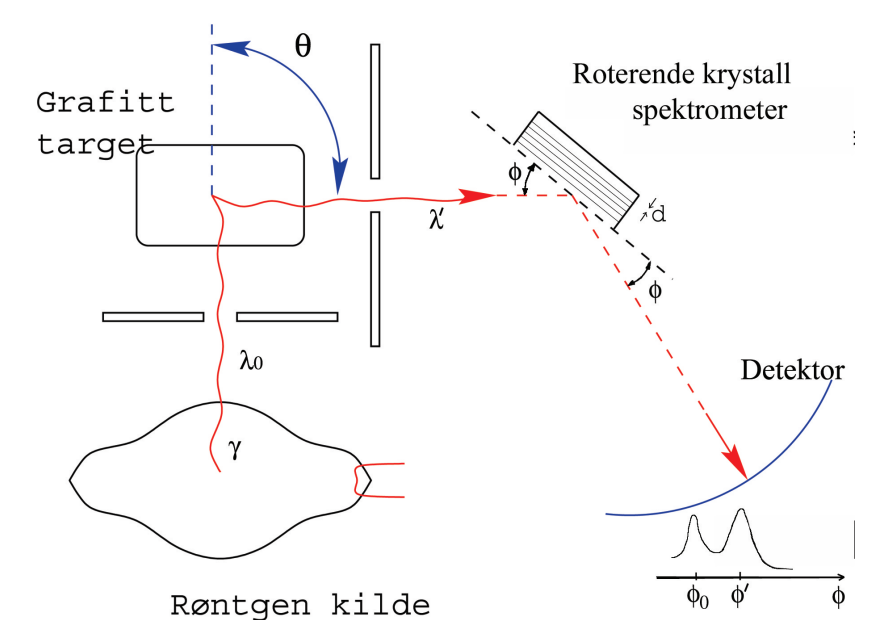
\includegraphics[scale = .4]{Figures/Compton oppsett.png}
  \caption{Oppsett av forsøk for Compton spredning}
  \label{fig: Compton oppsett}
\end{figure}

Vi sender Röntgenstråling med energi $E_0 = hν = h c / λ_0$ en hvis bølgelengde, på et mål laget av grafitt. Det kolliderer med elektronene i materialet, og skyter ut et nytt foton med ca. samme bølgelengde og energi. Dette fotonet kolliderer i krystall spektrometeret. Krystallen har flere lag som fotonet kan kollidere med. Flere fotoner kan da ha konstruktiv interferens med hverandre gitt ved $nλ = 2d \sin ϕ$, der d er tykkelsen på krystallen, $n$ er et heltall og at $ϕ$ er innfallsvinkelen. Noen ganger kommer det et fotonet med større bølgelengde og dermed mindre energi. Denne spredningen av fotonene sin energi som sett nederst til høyre i figur \ref{fig: Compton oppsett} kalles Compton spredning. En fant også ut at hvis en endrer vinkelen $θ$ fra 90 grader til 45 grader skaper en større spredning som sett i \ref{fig: Compton resultater}. 

\subsection{Forklaring}

\begin{figure}[h!]
  \centering
  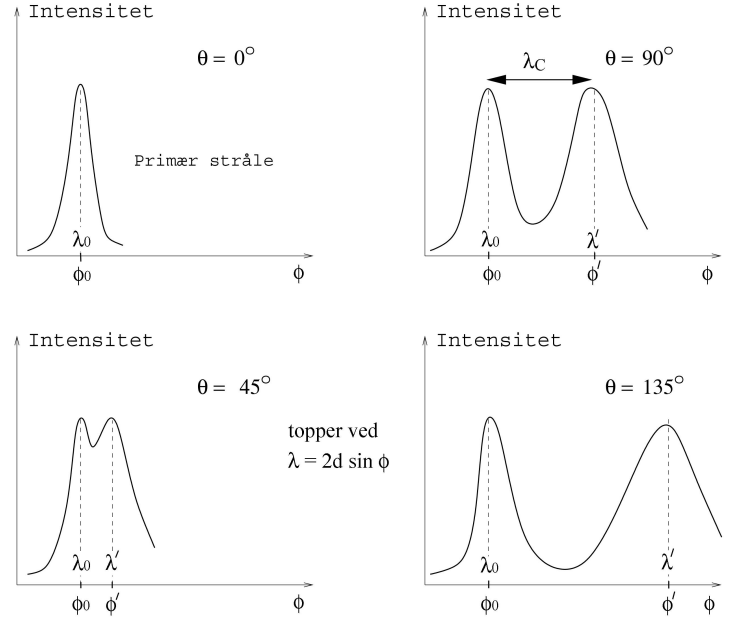
\includegraphics[scale = .5]{Figures/Compton resultater.png}
  \caption{Resultat ved compton eksperiment}
  \label{fig: Compton resultater}
\end{figure}

Einstein forstod at hvis energien til fotonet var redusert måtte det også bety en reduksjon i bevegelsesmengde HVIS en er på fotonet som en partikkel. Han mente fotoner har følgende egenskaper: 
\begin{enumerate}
    \item $E = høn = h c / λ$
    \item $E = mc^2 \frac{1}{\sqrt{1 - v^{2} / c^{2}}} ⇒ v = c, \quad m = 0$
    \item $E = \sqrt{p^{2} c^{2} +(mc^{2})^{2}} ⇒ p = E /c = hν / c = h /λ$
\end{enumerate}
Einstein tenkte da at energi og bevegelsesmengde må være bevart. Hvis en tenker at elektronene står stille vil da fotonet ha bevegelsesmengde $p_{γ_{x}}$ og $p_{γ_{y}}$ og elektronet bevegelsesmengde $p_{e} = 0$ 




\subsubsection*{Før}
Foton: 
\begin{itemize}
    \item $E_{γ} = h c / λ_0$
    \item $p_{γ_{x}} = h / λ_0$
    \item $p_{γ_{y}} = 0$  
\end{itemize}

Elektron
\begin{itemize}
    \item $E_{e} = m_e c^{2}$
    \item $p_e = 0$
\end{itemize}

\subsubsection*{Etter}
Foton: 
\begin{itemize}
    \item $E_{γ}' = h c / λ'$
    \item $p_{γ_{x}}' = h / λ' \cos θ$
    \item $p_{γ_{x}}' = -h / λ' \sin θ$
\end{itemize}

Elektron: 
\begin{itemize}
    \item $E_{e}' = \sqrt{p^{2} c^{2} + m_e^{2}c^{4}}$
    \item $p_{e_{x}}' = p_e' \cos ζ$
    \item $p_{e_{y}}' = p_e' \sin ζ$
\end{itemize}
  

\begin{figure}[h!]
  \centering
  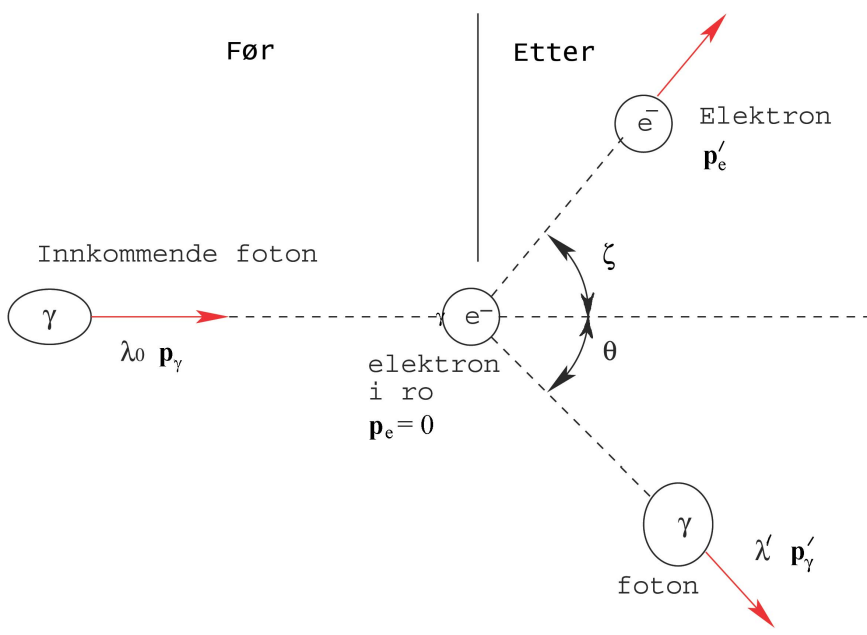
\includegraphics[scale = .5]{Figures/kollisjon elektron og foton.png}
  \caption{Kollisjon mellom elektron og foton}
  \label{fig: kollisjon elektron og foton}
\end{figure}


\[
\frac{hc}{λ_0} + m_e c^{2} = \sqrt{p^{2} c^{2} + m_e^{2}c^{4}} + \frac{hc}{λ'}
\]
\[
\left( \frac{hc}{λ_0} - \frac{hc}{λ'} + m_e c^{2}  \right)^{2} = p^{2} c^{2} + m_e^{2}c^{4}
\]
\[
\frac{h^{2}c^{2}}{λ_0^{2}} + \frac{h^{2}c^{2}}{λ'^{2}} - 2 \frac{h^{2}c^{2}}{λ_0 λ'} + \cancel{m_e^{2} c^{4}} + 2 m_e c^{2} \left( \frac{hc}{λ_0} - \frac{hc}{λ'} \right) = p^{2} c^{2} + \cancel{m_e^{2}c^{4}}
\]

\[
Δ λ = ( λ' - λ_0) = \frac{h}{m_e c} (1 - \cos θ)
\]
Som en konsekvens av ligningen over ser vi at maksimal spredning kommer av en vinkel $θ = 180^{\text{o}}$. 

Compton's Bølgelengde defineres som:
\[
λc = \frac{hc}{m_e c^{2}} = 0.00243 \text{ nm}
\]
\[
Δ λ_{\text{max}} = 2 λ_c = 0.0048 \text{ nm}
\]
Som vi ser i figur \ref{fig: Compton resultater} ser vi at uavhengig av spredning vil vi få samme $λ_0$ som tilsvarer en $ϕ_0$. Dette er fordi at fotonet også kan treffe store atomer som beveger seg ekstremt lite. \colorbox{red}{Hvilken av toppene tilsvarer hvilken type kollisjon ?}
\chapter{Bohr's Atommodell}
\section{05 Forelesnings Notater}
\subsection{Bohr's Atommodell}
\paragraph*{Balmer's empiriske parametrisering}
\[
λ = B\frac{n^{2}}{n^2 - 2^2}, \quad n = 3, 4, 5, \dots \qquad B = 3.64.6
\]
\paragraph*{Rydberg's generaliserte parametrisering}
\[
\frac{1}{λ} = R_h \left( \frac{1}{n^{2}_{f}} - \frac{1}{n_i^{2}} \right), \quad n_i = 2, 3, \ldots = \text{initial tilstand} \quad n_f = 1 \ldots n_i - 1 = \text{final tilstand}
\]

\[
λ = \underbrace{\frac{4}{R_h}}_{B} \left( \frac{n^{2}}{n^{2} - 2^{2}} \right) 
\]
\subsubsection{Thomson's Atommodell}
Atomet er en kule med en positiv kjerne og negative ladninger fordelt jevnt rundt kula. Ladningene er like store og har en ladning på $-e$.

\subsubsection{Rohterford's Atommodell}

Han testet med å skyte $α$- partikler og målte hvor den endte opp. Hadde atomet vært slik Thomson mente, ville det vært en jevn fordeling av lading i atomet. Det som skjedde var at noen $α$-partikler endret skarpt retning som hinter til at den positive ladningen er sentrert i midten av atomet. Hvis dette skal stemme kan ikke elektronene være så nære hverandre som først anstatt. Ettersom elektronene vil bli tiltrukket av den positive kjernen må de ha en hastighet for å motvirke de magnetiske kreftene. En ladning som akselerer vil sende ut lyst. Elektronene vil ha sentripetal akselerasjon som vil minke ettersom den mister energi i form av lys. Dette var under antagelsen at elektronene sender ut en kontinuerlig mengde lys. 

\subsubsection{Bohr's Atommodell}
Bor mente vi har en positiv kjerne med lading $Q = +e$ og et elektron i bane rundt med landing $-e$. 

\paragraph{Antagelser}
\begin{enumerate}
    \item Elektronet beveger seg i sirkulære baner om kjernen. Kraften mellom $e^{-}$ og kjernen er Coulomb Kraften.\\ Potensialet til elektronet er $\displaystyle  V(r) = -\frac{e^{2}}{4\pi\epsilon_{0}r}$.
    \item Bare visse elektron baner er stabile. 
    \item Elektromagnetisk stråling sendes ut dersom elektronets tilstand endres fra en bane til en annen. 
    \item Elektronbanene er bestemt av angulært momentum som er kvantisert. Elektronene har en sirkulær bane med en hastighet og akselerasjon.\\\\ 
    Kraften $\displaystyle  F = - \frac{\mathrm{d}U_e}{\mathrm{d}r}$ hvor $U_e$ er elektronets potensielle energi. Videre blir \\ $\displaystyle -\frac{\mathrm{d}U_e}{\mathrm{d}r} = k_e \frac{e^{2}}{r^{2}} $. \\\\ Ettersom kraften $F$ er sentripetalakselerasjonen kan vi finne hastigheten. \\\\ 
    $\displaystyle k_e \frac{e^{2}}{r^{2}} = \frac{mv^{2}}{r}$\\\\
    Den kinetiske energien $E $ blir da \\ 
    $\displaystyle K_e + U_e = \frac{mv^{2}}{2} - k_e \frac{e^{2}}{r}$

    
\end{enumerate}
\subsubsection{Klassisk fysikk Coulomb-vekselvirkning}
Potensiell energi \\\\ 
$\displaystyle U_e = -k_e \frac{e^{2}}{r}$ \\\\
Kraft \\\\
$\displaystyle F_e = k_e \frac{e^{2}}{r^{2}} = \frac{m_e v^{2}}{r}$\\\\
Energi \\\\
$\displaystyle E = K_e + U_e = - k_e \frac{e^{2}}{2r}$\\\\ 
Spin \\\\
$\displaystyle \vec{L} = \vec{r} × \vec{p} = r × m \vec{v} = rmv = nℏ $. \\\\
Observerer at $\displaystyle  mv^{2} = m \frac{n^{2}ℏ^{2}}{r^{2} m^{2}} = k_e \frac{e^{2}}{r}$.\\\\
$\displaystyle mv^{2} = \frac{1}{r} = k_e \frac{e^{2}m}{n^{2}ℏ^{2}}$. \\\\
$\displaystyle E = -k_e e^{2} \frac{e^{4} mc^{2}}{2 ℏ^2 c^2 n^2}$\\\\.
Setter in verdier for hydrogen atom
$\displaystyle E_n = -\frac{\left( 1.44 \text{ eVnm} \right) ^{2} 0.511 \text{ MeV}}{2\left( 197.3 \text{ eVnm} \right)^2 } \frac{1}{n} = -13.61 \frac{1}{n^2} \text{ eV}$\\\\ som gir energien til et elektron i et hydrogen atom avhengig av skallet $n = 1, 2, 3\ldots$.   

\[
E_f - E_i = - 13.6 \left( \frac{1}{n^2 _{f} - \frac{1}{n_i^2}} \right) \text{ eV} = E_{γ} = hν = hc/λ
\]
\[
\frac{1}{λ} = \underbrace{\frac{-13.5}{hc}}_{R_h} \left( \frac{1}{n_f ^2} - \frac{1}{h^2} \right) 
\]
Denne modellen viser at lysets sender ut diskré energier. 

En observerte at atomene i atmosfæren absorberte lys med en bestemt frekvens. Dette var i samsvar med Bohr's atommodell.


\subsection{Franck-Hertz eksperimentet}

\begin{figure}[h!]
  \centering
  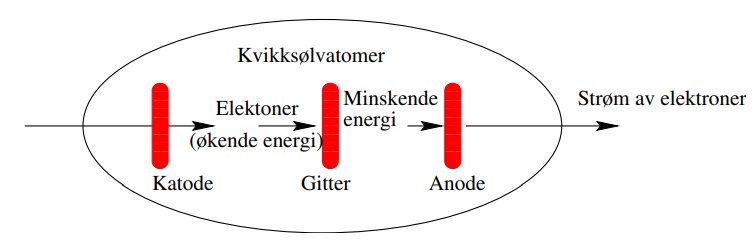
\includegraphics[scale = .7]{Figures/Franck-Hertz Eksperiment.png}
  \caption{Franck Hertz eksperimentet}
  \label{fig: Frank Hertz}
\end{figure}
Ved gitteret er det positivt potensialet som blir negativt mot katoden og anoden. Den totale spenning $V$ er gitt ved 
\[
V = V_{\text{KG}} - I V_{\text{GA}}I
\]
Elektronene Reiser fra Katoden og mister litt energi over gitteret. Mister de for mye energi vil de ikke kunne komme seg til anoden. Hvis spenningen øktes vil kollisjonen i gitteret ha mindre effekt og det øker sjansen for å komme seg til anoden. Dette varer frem til spesifikk spenninger hvor vi ser en dip i antall elektroner som når frem til anoden. Dette er fordi at elektronene får nok energi til å eksitere elektronene i atomene i gitteret, og mister dermed ekstremt mye mer energi enn vanlig. Noen elektroner vil likevel kunne både eksitere og komme seg til anoden. Ved å øke spenningen enda mer vil vi på nytt se en reduksjon av strøm ettersom elektronene eksiterer enda et elektron i et nytt atom i gitteret. De eksiterte elektronene vil falle ned til sin grunntilstand i et laver skall og vil sende ut ut energien i form av lys. 

\paragraph{Oppsumering}
\begin{itemize}
    \item Antar eksistensen av stasjonære tilstander
    \item Antar at elektronet i de sirkulære banene, og da er angulærmomentum kvantisert med $L = mvr = n ℏ$
    \item Lyktes spektakulært med å forutsi atomspekteret og de kjemiske egenskapene til enkle atomer 
    \item Idéen om elektronbaner blir modifisert av kvantemekanikken
\end{itemize}

\chapter{Materiens Bølgeegenskaper}
\section{06 Forelesnings Notater}
\paragraph{\underline{Sentrale Kunnskaper}}
\begin{itemize}
    \item Beskrive de Broglies hypotese og forstå hvordan de Broglies teori bidrar til Bohr's atommodell
    \item Beskrive resultatene fra dobbelspalte-eksperimentet 
    \item Beskrive hvordan eksperiment viser på partikkel- og bølge-egenskaper til materien
    \item Forstå sannsynligheten til treff, og interferensmønster på skjermen bak. 
    \item Beskrive interferensfenomenet i Davisson-Germer eksperimentet og Thomson-diffraksjon. 
\end{itemize}

\subsubsection{de Broglies hyptotese og atom}
\paragraph{Hypotese}
Hvis lys/fotoner oppfører seg som både bølge og partikkel må det samme gjelde materie. 

Da må materie ha en energi $E$ og en bevegelsesmengde $ρ$. Vi ser på dette i kontekst av elektroner 
\[
E = hν = ℏω, \quad ω = 2πν \text{ (vinkelfrekvens)}
\]
\[
ρ = \frac{h}{λ} = ℏk, \quad k = \frac{2π}{λ} \text{ (bølgetall)} 
\]
\[
nλ  = \underbrace{2πr}_{\text{omkrets}} 
\]
Det betyr at omkretsen til sirkelen er en multippel av bølgelengden $λ$. 

Vi slår sammen bølgeversjonen av bevegelsesmengde og partikkel versjonen av bevegelsesmengde.
\paragraph{Bølge} 
\[
ρ = \frac{h}{λ} = ℏk = \frac{h}{2πr}n = ℏn = mv ⇒ ℏn = \underbrace{rmv}_{\text{Ang. momentum}} = L = ℏn
\]
Da er angulært moment også kvantisert. 

Vi vet fortsatt ikke nøyaktig \textit{hva} en partikkel er, men bare dets tilstand. 

\paragraph{Oppsumering}
\begin{itemize}
    \item Elektronet tilordnes både partikkel- og bølgeegenskaper. 
    \item Forklarer Bohr's kvantisering av angulærmomentum.
    \item Bølgeegenskapen er en fundamental forskjell mot Bohr's partikkel-lignende elektron. 
    \item Kvantisering av bølgelengden er det som gjør kvantisering av energien mulig. 
\end{itemize}


\subsubsection{Dobbeltspalte-eksperimentet}
Fenomenet kan bare forklares, ikke begrunnes. Kort oppsummert vil vi se et interferens mønster uavhengig av om vi sender ut bølger, eller kvantiserte energi pakker (fotoner) av elektromagnetisk stråling. Det har ikke noe å si hvor stort mellomrom mellom utskytningen av fotoner. Vi får uansett det samme mønsteret. Hvor hver partikkelen treffer på skjermen bak, er uavhengig av hverandre og helt tilfeldig. Hvorfor dette skjer? \underline{Vi vet ikke}. Dette kan gjennomføres med vannbølger, lydbølger, elektromagnetisk stråling, eller atomer. Hvis vi setter en sensor foran bare én av spaltene vil partiklene passere ca. halvparten av gangene, men interferens mønstrete opphører. 

\begin{itemize}
    \item Enkelt-partikler må dermed \textit{interferere} med seg selv. Som om det passerer gjennom begge spalter samtidig. 
    \item Hver partikkel har en eget innebygd sannsynlighet. 
    \item Vi vet ikke hvilken vei det passerer gjennom spaltene, eller om det er begge samtidig. 
    \item Etter treff, vet vi heller ikke hvilken vei det tok.
    \item Målingen av banen til partikkelen ⇒ interferens opphører. 
    \item Måling endrer sannsynligheten. 
    \item Partikkelen vet ikke selv hvilken vei det skal ta. 
\end{itemize}

\paragraph{Hidden variables - teorien}
Partikkelen må selv vite hvilken spalte den skal gjennom, og den er da underkastet en deterministisk oppførsel. Vi kjenner bare ikke den underliggende fysikken. \\\\
"\textit{Gud spiller ikke terning}" \\- Albert Einstein. \\\\
"\textit{"Slutt å fortelle Gud hva han skal gjøre}" \\- Niels Bohr. 

\subsubsection{Sanssynlighetstettheten}
\[
\frac{\mathrm{d}^2 Ψ(x)}{\mathrm{d}x^2} = E ⋅ Ψ (x)
\]


\section{07 Forelesnings notater}
\subsection{Oppdagelsen av Schrödinger-ligningen}
\paragraph{\underline{Sentrale kunnskaper}}
\begin{enumerate}
    \item Skissere og motivere Schrödinger-ligningen fra Maxwells ligning. 
    \item Taylors rekkeutvikling spesielt på relativistisk energi. 
    \item $(fg)'' = f''g + 2f'g' + fg''$
    \item Løse $\displaystyle \left( iℏ \frac{∂ }{∂ t} + \frac{ℏ^{2}}{2m}\frac{∂^2 }{∂ x^2} \right) Ψ(x,t) = 0 $
    \item Superposisjon: Forstå hvordan man lager en bølgepakke av planbølger, og beregne gruppe- og fase-hastighet 
\end{enumerate}
\subsubsection{Davisson-Germer-eksp.}
Sender inn elektroner i en nikkel krystall, som reflekteres på i en fast vinkel $ϕ$. Uavhengig om man sendte inn et eller flere elektroner ble det interferens. Da må man kunne se på elektronet som en bølge. Konstruktiv interferens må da være gitt ved 
\[
nλ = 2d\sin(ϕ).
\]
\subsubsection{Thomsons elektrondiffraksjon}
\paragraph{Vannbølge}
Har en intensitet $I = A^2$ hvor $A$ er amplituden.

\paragraph{Elektromagnetisk bølge}
Har en intensitet $I \propto ϵ(x, y, t)^2 $ hvor $\epsilon$ er elektromagnetisk feltstyrke.

\paragraph{Maxwells likninger på flere former}
\[
\left( \frac{∂^2 }{∂ t^2} - c \frac{∂^2 }{∂ x^2} \right) ϵ (x,t) = 0
\]
\[
∇ × ϵ = - \frac{∂ \vec{B}}{∂ t}
\]
\[
\oint_{C} ϵ \ \mathrm{d}l =- \frac{∂ }{∂ t} \oiint  \vec{B} \mathrm{d}S 
\] 
\[
ϵ (x,t) = ϵ_0 e^{i(kx - ωt)}
\]
\paragraph{Kvantemekanisk}
\[
E_{γ} = hν
\]
\[
I = \left( \frac{∂^2}{∂ t^2} - c \frac{∂^2 }{∂ x^2} \right) Ψ(x,t) = 0
\]
\[
Ψ(x,t) = Ψ_0 e^{i(kx - ωt)}
\]
\[
I = \frac{\text{Antall fotoner}}{s ⋅ A} = \left| Ψ(x,y,t) \right| ^2
\]
Hvis ligningen for intensiteten gjelder for en gruppe fotoner må det også gjelde for et enkelt foton. Fotoner interagerer ikke med hverandre derfor vet vi dette. For et individuelt foton er det derfor slik at bølgefunksjonen kvadrert er sannsynligheten for at et elektron treffer et punkt på skjermen. Hvis vi integrere dette får vi 1 ettersom vi integrer sannsynligheten. Den er dermed normalisert. 
\[
∫ \left| Ψ(x,t) \right|^2 \ \mathrm{d}x  = 1
\]

\paragraph{Foton}
\[
\left( \frac{∂^2 }{∂ t^2} - c^2 \frac{∂^2 }{∂ x^2} \right) Ψ(x,t) = 0, \qquad Ψ(x,t) = Ψ_0 e^{i(kx - ωt)} = Ψ_0 e^{i(px -Et) / ℏ}, \quad p = ℏk, \quad E = ℏω
\]
\[
\left( \frac{i}{ℏ^2} \right)^2 \left( \underbrace{ \left( -E \right) ^2 - c^2 p^2}_{0}\right) Ψ_0 e^{i(px -Et) / ℏ} = 0, \qquad E = pc, \quad E^2 = c^2 p^2
\]

\paragraph{Partikkel med masse $m > 0$}
\[
E^2 = p^2c^2 + m^2c^4 
\]
Antar $Ψ = Ψ_0 e^{i(px - Et)/ℏ}$. 
\[
\left( \frac{i}{ℏ} \right) ^2 \left( \left( -E \right) ^2 - c^2p^2 \right) Ψ_0 e^{i(px - Et) / ℏ} = 0
\]
\[
\left( \frac{i}{ℏ} \right) ^2 \left( \underbrace{p^2c^2 + m^2c^4 - c^2p^2}_{≠ 0} \right) Ψ_0 e^{i(px - Et) / ℏ} = 0
\]
Dette går ikke opp. Vi mangler et ledd med $-m^2c^4$. 
\[
\left( \frac{∂^2 }{∂ t^2} - c \frac{∂^2 }{∂ x^2} - \frac{1}{ℏ^2} \right) Ψ(x,t) = 0, \qquad Ψ(x,t) = Ψ_0 e^{i(px - Et) / ℏ}
\]
\[
\left( \left( - \frac{iE}{ℏ} \right)^2  - c^2 \left( \frac{ip}{ℏ} \right)^2 + \frac{1}{ℏ}m^2c^4  \right) Ψ(x,y) = 0
\]
\[
\left( \underbrace{- \frac{1}{ℏ^2} \left( p^2c^2 + (mc^2)^2  \right) + \frac{c^2p^2}{ℏ^2} + \frac{1}{ℏ^2}m^2c^4 }_{0}\right)   Ψ(x,t) = 0
\]
\[
E^2 = p^2c^2 + (mc^2)^2
\]
\[
E = \sqrt{p^2c^2 + (mc^2)^2} = mc^2 \sqrt{1 + \frac{p^2c^2}{\underbrace{mc^2}_{x}}}
\]
Kjører Taylor utvikling. 
\[
E = mc^2 \left( 1 + \frac{1}{2} \frac{p^2c^2}{(mc^2)^2} + \frac{1}{8}\ldots    \right) 
\]
\[
E = mc^2 + \frac{1}{2} \frac{p^2}{m} = \underbrace{\frac{p^2}{2m}}_{E_k} + \underbrace{mc^2}_{E_0}
\]
\[
p = mv, \quad \frac{p^2}{2m} = \frac{mv^2}{2}
\]
\[
E = E_k + E_0, \qquad Ψ = Ψ_0 e^{i(px - Et) / ℏ}
\]
\[
\left( \left( - \frac{iE}{ℏ} \right)^2  - c^2 \left( \frac{ip}{ℏ} \right)^2 + \frac{1}{ℏ}m^2c^4  \right) Ψ(x,y) = 0
\]
Setter inn nytt utrykk for energi 
\[
    - \frac{1}{ℏ^2}\left(\underbrace{\left( \frac{p^2}{2m} + mc^2 \right) ^2 - p^2c^2 + (mc^2)^2}_{≠ 0} \right) Ψ(x,t) = 0
\]
Det fungerer ikke å bare bytte ut utrykket for energi. 
\[
Ψ = Ψ_0 e^{i(px - E_k t - E_0 t) / ℏ}
\]
\[
\underbrace{e^{-iE_0t / ℏ}}_{θ}\quad \underbrace{Ψ_0 e^{i(px - E_k t) / ℏ}}_{Ψ_k} = 0
\]

\[
\left( \frac{∂^2 }{∂ t^2} - c^2 \frac{∂^2 }{∂ x^2} + \frac{(mc^2)^2}{ℏ^2} \right) θ(t) Ψ_k(x,t) = 0
\]
\[
Ψ_k \frac{∂^2}{∂ t^2} θ + 2 \frac{∂ }{∂ t}θ \frac{∂ Ψ_k}{∂ t} + θ\frac{∂^2 }{∂ t^2}Ψ_k - c^2 \frac{∂^2 }{∂ x^2} θ Ψ_k + \frac{(mc^2)^2}{ℏ^2} θ Ψ_k 
\]
\[
\cancel{Ψ_k \left( \frac{-iE_0}{ℏ} \right) ^2 θ} + 2 \left( \frac{-iE_0}{ℏ} \right) θ \frac{∂ }{∂ t}Ψ_k + θ c^2 \frac{∂^2}{∂ x^2} Ψ_k + \cancel{\frac{(mc^2)^2}{ℏ^2} θ Ψ_k}
\]
\[
2 \left( \frac{-iE_0}{ℏ} \right) \frac{∂ Ψ_k}{∂ t} + \frac{∂^2 Ψ_k}{∂ t^2} - c^2 \left( \frac{ip}{ℏ} \right) Ψ_k
\]
\[
2 \left( \frac{-iE_0}{ℏ} \right) \left( \frac{-iE_0}{ℏ} \right) Ψ_k + \left( \frac{-iE_0}{ℏ} \right) ^2 Ψ_k + c^2 \frac{p^2}{ℏ^2} Ψ_k
\]

\[
-2E_0 E_k Ψ_k - E_k ^2 Ψ_k + mc^2 \frac{p^2}{2m}Ψ_k
\]
\[
\left( -2E_0 E_k - E_k ^2 +  2 E_0 E_k\right) ψ_k ≠ 0
\]
Dette går ikke opp. La oss ta bort ledde som ødelegger
\[
2 \left( \frac{-iE_0}{ℏ} \right) \frac{∂ Ψ_k}{∂ t} - c^2 \frac{∂^2 Ψ_k}{∂ x^2} = 0
\]
\[
2 \left( - \frac{i m c^2}{ℏ} \right) \frac{∂ Ψ_k}{∂ t} - c^2 \frac{∂^2 Ψ_k}{∂ x^2} = 0
\]
\[
iℏ \frac{∂ Ψ_k}{∂ t} + \frac{ℏ}{2m} \frac{∂^2 Ψ_k}{∂ x^2} = 0
\]
Dette er Schrödingerligningen for frie partikler

\section{08 Forelesnings Notater}
\paragraph{\underline{Sentrale kunnskaper}}
\begin{enumerate}
    \item Forholdene i tabell 1.4 i kompendiet 
    \item Beregne forventningsverdi og standardavvik for diskrete og kontinuerlige variabler
    
    \item Forstå superposisjon som for frie partikler er oppbygget av planbølger
    \item Hva som skjer når man måler en superposisjon av tilstander 
    \item Københavnstolkningen 
\end{enumerate}

Den vanlige maxwell likningen fungerer ikke når vi setter inn partikkelegenskapene til fotonet. Vi får et restledd på $\displaystyle \left( mc^2 \right) ^2$ som gjør at den fulle likningen ikke lenger er null. Vi ser at hvis vi legger til en faktor av $\displaystyle - \left( \frac{i}{ℏ} \right) \left( mc^2 \right) ^2$ ved å ta hensyn til hvileenergien før vi deriverer og likningen løser seg. 

\subsection{Tidsavhengige bølgeligninger}
\paragraph{Maxwells ligning for klassiske elektromagnetiske bølger (relativistisk)}
\[
\left( \frac{∂^2 }{∂ t^2} - c^2 \frac{∂^2 }{∂ x^2} \right) ϵ(x,t) = 0
\]
\paragraph{Klein-Fock-Godronds relativistiske lignign for frie partikler med masse (spinn løse)}
\[
    \left(\frac{∂^2 }{∂ t^2} - c^2 \frac{∂^2 }{∂ x^2} + \left(\frac{mc^2}{ℏ}\right)^2\right) Ψ(x,t) = 0
\]

\subsection{Bølgepakke for fri partikkel}
\[
\left(-i ℏ \frac{∂ }{∂ t} - \frac{ℏ^2}{2m} \frac{∂^2 }{∂ x^2} \right) Ψ(x,t) = 0
\]
\subsection{Generell løsning av bølgepakke av planbølger}
\[
Ψ(x,t) = \sum_{n}^{} c_n e^{i \left( k_n x - ω_n t  \right) }
\]
Kan også skrives 
\[
Ψ = \sum_{n}^{} c_n e^{i \left( p_n x - E_n t \right)/ℏ}
\]
\[
ψ = \sum_{n}^{} c_n e^{i \left( k_n x - ω_n t \right)}
\]
Her er $\displaystyle k_n = \frac{2π}{λ} = \frac{p}{ℏ}\quad , \quad ω = \frac{2πc}{λ} = \frac{E}{ℏ}$. 
\paragraph{Superposisjonering av egentilstander}
En bølgefunksjon er en superposisjon av egentilstander. Hvis vi måler bølgen kollapser den til en enkelt bølge med bestemt energi, bevegelsesmengde og bølgelengde. Hvordan dette skjer vet vi ikke. Konstanten $\left|c_n\right|^2 $ er sannsynligheten for kollaps til planbølgen med $λ_n = 2π / k_n$. Da følger det naturlig at $\left|c_n\right|^2 = 1$

\subsection{Tolkninger}
\paragraph{Realist}
Partikkelen hadde en forutsagt bane før måling og det er en skjult variabel som styrer dette. (Har blitt motbevist)
\paragraph{Ortodoks / Københavnstolkningen}
Bølgefunksjonen er ikke ekte. Målingen fikk den til  å kollapse. Målingen påvirker partikkelen, uten den også 
\paragraph{Agnostisk}
Har ikke noe å si ettersom vi må måle uansett
\newline \newline
Den mest aksepterte tolkningen er Københavnstolkningen. 

\section{09 Forelesnings Notater}
\paragraph{\underline{Sentrale kunnskaper}}
\begin{itemize}
    \item Forså begrepet sannsynlighetstettheten $\left| Ψ(x,t) \right| ^2$ for en partikkel og at $\left| Ψ(x,t) \right| ^2 δx$ er sannsynligheten for å finne en partikkel mellom $x$ og $x + δx$
    \item Normalisere bølgefunksjonen $\left| Ψ(x,t) \right| ^2$ og vise at den er tidsuavhengig. 
    \item Beregning av $\left< x \right>, σ,...$
    \item Beregne posisjon og bevegelsesmengde for en partikkel via bølgefunksjonen
\end{itemize}

\paragraph{Forventningsverdi}
\[
\left< j \right> = ∑_{j=1}^{n} j ⋅ P_N(j)
\]
Med et standard avvik $σ$ for et kast $j - \left< j \right>$ gitt ved
\[
σ = \sqrt{\left<\left(j - \left<j\right>\right)^2\right>} = \sqrt{∑_{j=1}^{n} \left(j - \left<j\right>\right)^2 ⋅ P_N(j)} = \sqrt{\left<j^2\right> - \left<j\right>^2}
\]
\subsubsection*{Viktig om bølgefunksjonen}
\begin{enumerate}
    \item $Ψ$ er en generell løsning for gitt $v(x)$
    \item $Ψ → 0$ når $x → ± ∞$
    \item $Ψ$ og $\frac{\mathrm{d}Ψ}{\mathrm{d}x}$ må være kontinuerlige
    \item $\left| Ψ \right| ^2 = Ψ ⋅ Ψ^{*}$ er en sannsynlighetstettheten
    \item $∫_{a}^{b} \left| Ψ \right| ^2 \ \mathrm{d}x$ er sannsynligheten for å finne en partikkel mellom $a$ og $b$. 
    \item $∫_{-∞}^{∞} \left| Ψ \right| ^2 \ \mathrm{d}x = 1$ er avhengig av tid
\end{enumerate}

Hvis $Ψ$ er tidsuavhengig må den den deriverte være konstant. 
\[
\frac{\mathrm{d}}{\mathrm{d}t} ∫_{-∞}^{∞} Ψ^{*}Ψ  \ \mathrm{d}x = ∫ \frac{\mathrm{d}}{\mathrm{d}t} Ψ^{*} Ψ \mathrm{d}x = 0
\]
\[
∫ \frac{\mathrm{d}}{\mathrm{d}t} Ψ^{*} Ψ \mathrm{d}x = ∫ \underbrace{Ψ^{*} \frac{∂ Ψ}{∂ t} + \frac{∂ Ψ^{*}}{∂ t} Ψ}_{P} \mathrm{d}x = 0        
\]  
\[
P = Ψ^{*} \frac{1}{iℏ} \left( - \frac{ℏ^2}{2m} \frac{∂^2 }{∂ x^2} + V \right) Ψ + \frac{1}{iℏ} \left( - \frac{ℏ}{2m} \frac{∂^2 }{∂ x^2} + V \right) Ψ^{*} Ψ = 0
\]
\[
\frac{iℏ}{2m} \left( \frac{∂^2 Ψ}{∂ x^2}Ψ^{*} - \frac{∂^2 Ψ^{*}}{∂ x^2}Ψ \right) 
\]
\[
\frac{∂ }{∂ x} \left( Ψ^{*} \frac{∂ Ψ}{∂ x} - \frac{∂ Ψ^{*}}{∂ x}Ψ \right) = \cancel{\frac{∂ Ψ^{*}}{∂ x}} + Ψ^{*} \frac{∂^2 Ψ}{∂ x^2}Ψ^{*} - \frac{∂^2 Ψ^{*}}{∂ x^2}Ψ - \cancel{\frac{∂ Ψ^{*}}{∂ x}Ψ}
\]
Setter tilbake inn i $P$
\[
∫ \frac{iℏ}{2m} \frac{∂}{∂x} \left( \frac{∂ Ψ}{∂ x} Ψ^{*} - \frac{∂ Ψ^{*}}{∂ x} Ψ \right) \mathrm{d}x = \frac{iℏ}{2m} \left[ \frac{∂ Ψ}{∂ x} Ψ^{*} - \frac{∂ Ψ^{*}}{∂ x} Ψ \right]_{-∞}^{∞} = 0 
\]

\subsection{Forventningsverdi og Standardavvik for Partikler}
\[
\left< x \right> ∫_{-∞}^{∞} x \left| Ψ(x,t) \right|^2  \ \mathrm{d}x
\]
\[
\left< x^2 \right> ∫_{-∞}^{∞} x^2 \left| Ψ(x,t) \right| ^2 \ \mathrm{d}x
\]
\[
σ_{x} = \sqrt{\left< x^2 \right> - \left< x \right>^2}
\]
Vi skal finne forventet bevegelsesmengde $\left< p \right>$. Da trenger vi en sannsynlighetsfunksjon $Φ(p,t)$for bevegelsesmengde.
\[
\left<p^2\right> = ∫_{-∞}^{∞} p^2\left|Φ(p,t)\right| ^2 \ \mathrm{d}p
\]
Klassisk fysikk: $p = mv = m \frac{\mathrm{d}}{\mathrm{d}t}x$
Kvantefysikk: $\left<p\right> = m \left<v\right> = m \left<\dot{x}\right>$
\[
\left<p\right> = m \frac{\mathrm{d}}{\mathrm{d}t} ∫ x Ψ^{*} Ψ \mathrm{d}x = m ∫ x \frac{∂ }{∂ t}Ψ^{*}Ψ \mathrm{d}x = m \frac{iℏ}{2m} ∫_{-∞}^{∞} x \frac{∂}{∂x} \left(Ψ^{*} \frac{∂ Ψ}{∂ x} - \frac{∂ Ψ^{*}}{∂ x}\right)  \ \mathrm{d}x
\]
Dette løses ikke like enkelt siden vi har en faktor av $x$. Vi må derfor integrere og får da følgende: 


\section{10 Forelesnings Notater}
\paragraph{\underline{Sentrale kunnkaper}}
\begin{enumerate}
    \item Sette opp og utlede løsning til TUSL for uendelig dyp brønn, beregne egentilstandene og forstå ortogonalitet og kronecker delta.
    \item Lage superposisjon av egentilstander
    \item Forstå figurer der vi kombinerer potensial, energi og bølgefunksjon, beregne $\left<h\right>, σ_{H}$ og sannsynligheten for å måle n-te tilstand
    \item Trig funksjoner, deres integrerte, deriverte og sum
\end{enumerate}

\subsection{Potensialet til uendelig dyp brønn}
\[
\hat{Q} → \hat{H} = \left(- \frac{ℏ^2}{2m}\frac{\mathrm{d}^2}{\mathrm{d}x^2} + V(x)\right) \quad , \quad Ψ_{E} ≡ Ψ_{n}(x,t) = ψ_n(x)f_n(t)
\]
Vi separerer bølgefunksjonen i to deler, en som er avhengig av posisjon og en som er avhengig av tid. 
\[
\hat{H}ψ_n(x) = E_nψ_n(x) \quad , \quad φ_n(t) = E^{-iE_{n} t / ℏ}
\]
\paragraph{Generell bølgefunksjon}
\[
Ψ(x,t) = \sum_{n=1}^{\infty}c_nψ_n(x)e^{-iE_nt/ℏ}
\]
Ettersom vi har separert tid og rom kan vi sette $t = 0$ for å gjøre om eksponenten til 1. Da blir bølgefunksjonen
\[
Ψ(x,0) = \sum_{n=1}^{}c_nψ_n(x) \quad , \quad ∑_{n}^{} \left|c_n\right|^2 = 1 = ∫ ψ^{*}_n(x)ψ_n(x,0)\ dx
\]
$\left|c_n\right|^2 $ er sannsynligheten for å måle n-te tilstand. Bølgefunksjonen er for abstrakt til å finne energien, men vi kan finne gjennomsnittsenergien $\left<H\right>$. 
\[
\left<H\right> = ∫ Ψ^{*}(x,t)\hat{H}Ψ(x,t)\ dx = ∑_{n}^{} E_n \left|c_n\right|^2
\]
Hvis alle tilstandene har samme energi kan dette faktoriserer ut og vi får. 
\[
Ψ(x,t) = \left(∑_{}^{} c_n ψ_n(x)\right)e^{-iE_nt/ℏ}
\]
\[
\left<p\right> = ∫ Ψ^{*}(x,t)\hat{p}Ψ(x,t)\ dx ≠  ∑_{n}^{} p_n \left|c_n\right|^2
\]
Det går ikke alltid å summere som vanlig når vi skal finne forventningsverdien til bevegelsesmengden $p$. 

\paragraph{Triks for å spare tid}
Annta et potensialet som variere, men er konstant i noen intervaller. Da vil TUSL gitt ved 
\[
\left(- \frac{ℏ^2}{2m}\frac{\mathrm{d}^2}{\mathrm{d}x^2} + V_0\right)ψ_n(x) = E_nψ_n(x)
\]
\[
- \frac{ℏ^2}{2m}\frac{\mathrm{d}^2}{\mathrm{d}x^2} ψ_n = \underbrace{\left(E_n - V_0\right)}_{K_n} ψ_n(x)
\]
\[
ψ_n(x) = A e^{i k_nx} + B e^{-i k_nx}
\]
\[
K_n = E - V_0 = \frac{ℏ^2 k_n^2}{2m} ⇒ k_n = \sqrt{\frac{2m}{ℏ^2}(E_n - V_0)}
\]
Dette er mulig ettersom TULS er lokal med hensyn på $x$. Konstantene A og B er globale for hele funksjonen. 
Vi har noen forskjellige cenario. 
\begin{enumerate}
    \item $E > V_0$\\
    Dette er det vanligste tilfellet. Da vil $k_n$ være reelt og $ψ_n(x)$ er planbølgen. 
    \item $E < V_0$\\
    her er $k_n$ imaginært $κ_n = i k_n = \displaystyle \sqrt{- \frac{2m(E- V_0)}{ℏ^2}}$ som er reelt.\\
    $ψ_n(x) = \underbrace{A e^{κ_n x} + Be^{-κ_n x}}_{\text{Reelle eksp. funk.}}$.\\ 
    Det er bare i et lite område hvor energien $E$ er mindre enn potensiell energi $V$ 
    \item $E = V_0$
    $ψ_n(x) = A + Bx$
\end{enumerate}

\paragraph{Cases}
\[
V(x) = 0 \quad , \quad 0 \le x \le a \quad , \quad V(x) = ∞
\]
Vi skal finne en bølgefunksjon som er kontinuerlig både i og utenfor brønn. I brønnen er funksjonen 
\[
ψ_n(x) = A e^{i k_nx} + B e^{-i k_nx}
\]
Utenfor er den 0. Vi løser deretter 
\[
ψ(0) = 0 ⇒ B = -A
\]
Så løser vi for grensene 
\[
ψ(a) = A e^{i k_na} - A e^{-i k_na} = A \left(e^{i k_na} - e^{-i k_na}\right)
\]
Dette kjenner vi igjen som en sinus funksjon. 
\[
2iA\sin (k_na) = 0 ⇒ k_n = \frac{nπ}{a} \quad , \quad n = 1, 2, 3 \ldots , ∞
\]
\[
E_n = \frac{ℏ^2 k_n^2}{2m} = \frac{h^2}{2m} \frac{π^2}{a^2}n^2
\]
Vi normaliserer sinus funksjonen på følgende måte. 
\[
C \sin (k_na) = 0
\]
\[
1 = ∫ ψ_n^{*}ψ_n \ \mathrm{d}x = ∫_{0}^{a} C \sin (k_nx) ⋅ C \sin (k_nx) \ \mathrm{d}x = C^2 ∫_{0}^{a} \sin ^2 (k_n x) \ \mathrm{d}x
\]
\[
1 = C^2 \left.\left(\frac{x}{2} - \frac{1}{4 k_n} \sin (2 k_nx)\right)\right\rvert_{0}^{a} = C^2 \left(\frac{a}{2}\right) ⇒ C = \sqrt{\frac{2}{a}}
\]
Dette gir bølgefunksjonen
\[
ψ_n(x) = \sqrt{\frac{2}{a}} \sin \left(\frac{nπ}{a}x\right) \quad , \quad n = 1, 2, 3 \ldots 
\]
Egenfunksjonene er ortogonale og produktet vil alltid være 0, hvis ikke de har samme tilstand. 
\[
δ_{nm} = \begin{cases}
  1, &\text{ if }n = m\\
  0, &\text{ if }n ≠  m
\end{cases}
\]
En grei regel er at
\[
E_1 = \frac{ℏ^2 k^2}{2m} \frac{π^2}{a^2} \ \quad , \quad E_2 = E_1 ⋅ 2^2 \quad , \quad E_3 = E_1 ⋅ 3^2 \quad , \quad E_4 = E_1 ⋅ 4^2 \quad , \quad \ldots
\]
Da kan vi finne bølgefunksjonen
\[
Ψ(x,0) = ∑_{n}^{} c_n ψ_n(x) = ∑_{n}^{} c_n \sqrt{\frac{2}{a}} \sin \left(\frac{nπ}{a}x\right)
\]
\paragraph{Typiske eksamensoppgaver}
\begin{enumerate}
    \item å lage $Ψ(x,0)$ fra egenfunksjoner. 
    \item Anta $Ψ(x,0)$ hva er sannsynligheten at vi får n-te tilstand ved måling? Da må vi beregne $c_n$. ved $\displaystyle c_n = ∫ ψ_n^{*}(x) Ψ(x,0) \ \mathrm{d}x \frac{2}{nπ} \left(1 - \cos \left(\frac{nπ}{2}\right)\right)$
\end{enumerate}

\[
Ψ(x,0) = 
\begin{cases}
    \sqrt{\frac{2}{a}} &\text{ når } 0 \le x \le a / 2 \\
    0              & \text{ ellers } 
\end{cases}
\]

De første tre tilstandene er mye mer sannsynlig enn resterende og er ofte nok for en god approksimasjon. 


\subsection*{Dirac-delta-funksjonen}
\[
δ(x-a) = 
\begin{cases}
  ∞, &\text{ if }x = a\\
  0, &\text{ if }x ≠  a 
\end{cases}
\]
\[
∫_{-∞}^{∞} δ(x-a) \ \mathrm{d}x = 1
\]
\[
∫_{-∞}^{∞} f(x) ϕ(x-a) \ \mathrm{d}x = f(a)
\]
\subsection*{Ortogonale Egenfunksjoner}
\[
∫ ψ_n^{*}(x) ψ_m(x) \ \mathrm{d}x = δ_{nm}
\]
\[
Ψ(x,0) = ∑_{n}^{} c_n ψ_n(x)
\]
\[
ψ_m = ∑_{n}^{} c_n ψ_n \quad , \quad c_n = \begin{cases}
  1, &\text{ når }m = n\\
  0, &\text{ ellers }
\end{cases}
\]
\[
1 = ∫ ψ_m^{*}(x) ψ_m(x) \ \mathrm{d}x \overset{\underset{\text{antar}}{}}{=} ∫ ψ_m^{*} ∑_{n ≠ m}^{} c_n ψ_n \ \mathrm{d}x = ∑_{n ≠ m}^{} c_n \underbrace{∫ ψ_m^{*}ψ_n \ \mathrm{d}x}_{δ_{mn}} = 0
\]

<<<<<<< HEAD:Course/FYS2140-Kvantefysikk.tex
\section{11 Forelesnings Notater}
\subsection*{Fri partikkel og energi tilstander}
\subsubsection*{Diskrete tilstander}
Vi vet at 
\[
∫_{-∞}^{∞} ψ_m^{*}ψ_n \ \mathrm{d}x = δ_{mn}
\]
Da er spørsmålet hva som gjelder for Kontinuerlige tilstander.


\subsubsection*{Kontinuerlig variabler}
\[
Ψ_k(x,0) = ∫ c(k) Ae^{ikx} \ \mathrm{d}k
\]
\[
c(k) = ∫ \underbrace{A}_{\frac{1}{\sqrt{2π}}}e^{-kx}Ψ(x,0) \ \mathrm{d}x
\]
\subsubsection*{For alle Dirac-ortogonale $Ψ_k$}
\[
∫ Ψ_k^{*}Ψ(x,0) \ \mathrm{d}x ⇒ dk' = ∫ c(k')δ(k-k') \ \mathrm{d}k' = c(k)
\]
Da er
\[
c(k) = ∫  Ψ_k^{*}Ψ(x,0) \ \mathrm{d}x
\]
\[
\left<H\right> = ∫ Ψ^{*}(x,0) \hat{H}Ψ(x,0) \ \mathrm{d}x = ∬ c^{*}(k')Ψ^{*}_k \ \mathrm{d}k' \hat{H} \int c(k)Ψ_k \ \mathrm{d}x
\]
\[
∬ E_k c^{*}(k')c(k) ∫ \underbrace{Ψ_k^{*}(x)Ψ_k(x) \ \mathrm{d}x}_{δ(k' - k)} \ \mathrm{d}k' \ \mathrm{d}k
\]
\[
∫ E_k c^{*}(k)c(k) \ \mathrm{d}k = ∫ E_k \left|c(k)\right|^2 \ \mathrm{d}k
\]
\[
\left<H\right> = ∫ E_k \left|c(k)\right|^2 \ \mathrm{d}k
\]
\subsubsection*{Dirac-delta-funksjon}
\[
δ(k' - k) = 
\begin{cases}
  ∞, &\text{ if }k' = k\\
  0, &\text{ if not }
\end{cases}
\]
\subsection*{Fri partikkel og }
\[
Ψ(x,t) = Ψ_k(x,t) Φ(x) \quad , \quad  Φ(x) = A e^{- 2πg^2 \left(k_0x - ω_0t\right)^2} \quad Ψ_k(x,t) = \frac{1}{\sqrt{2π}} e^{i(k_0x - ω_0t)}
\] 
\[
∫ ψ^{*}ψ \ \mathrm{d}x = ∫_{-∞}^{∞} \frac{A^2}{2πk}e^{-2ay^2} \ \mathrm{d}y = \frac{A^2}{2πk} \frac{1}{2g} ⇒ A = \sqrt{4πgk}
\]
\[
∫_{-∞}^{∞} ye^{-2ay^2} \ \mathrm{d}y = 0
\]
\[
∫_{-∞}^{∞} y^2e^{-2ay^2} \ \mathrm{d}y = \frac{1}{4a} \frac{1}{2g}
\]
\[
Ψ(x,t) = \sqrt{2gk}e^{iy - ay^2} = Be^{iy - a^2} \quad , \quad \left|Ψ(x,t)\right|^2 = B^2e^{2ay^2}
\]
\[
\frac{∂Ψ}{∂y} = \left(i - 2ay\right)Ψ
\]
\[
\frac{∂^2 Ψ}{∂ y^2} = (-2a + \left(i - 2ay\right)^2)Ψ = \left(-2a + \left(-1 + 4a^2y^2+ 4iay\right)\right)Ψ
\]
\[
\hat{p} = -iℏ \frac{∂}{∂x} = -iℏ \frac{∂}{∂y} \quad , \quad \hat{p}^2 = - ℏ^2k^2 \frac{∂^2 }{∂ y^2}
\]
\[
\left<x\right> = ∫ x \left|Ψ\right|^2 \ \mathrm{d}x = ∫ \frac{1}{k}(y + ω)B^2 e^2-2ay^2 \frac{\ \mathrm{d}y}{k} = \frac{B^2}{k^2} ωt \frac{1}{2g}
\]
\[
\left<x\right> = \frac{2g}{k} ωt \frac{1}{2g} = \frac{ω}{k}t = v ⋅ t
\]
\[
\left<x^2\right> = \frac{B^2}{k^{3}} ∫ \left(y^2 + ω^2t^2 + 2ylwt\right)e^{-2ay^2} \ \mathrm{d}y = \frac{B^2}{k^{3}}\left(\frac{1}{4a} \frac{1}{2g} + ω^2t^2 \frac{1}{2g}\right)
\]
\[
\left<x^2\right> = \frac{2g}{k^2}\left(\frac{1}{4 ⋅ 2πg^2} \frac{1}{2g}\frac{ω^2t^2}{2g}/\right) = \frac{1}{k^3}\frac{1}{8πg^2} + \frac{ω^2t^2}{k^2}
\]
\[
σ_{x} = \sqrt{\left<x^2\right> - \left<x\right>^2} = \sqrt{\frac{1}{k^2}\frac{1}{8πg^2} + \frac{ω^2t^2}{k^2} - \left(\frac{ω}{k}t\right)^2}
\]
\[
σ_{x} = \sqrt{\frac{1}{k^2}\frac{1}{8πg^2} + \frac{ω^2t^2}{k^2} - \frac{ω^2t^2}{k^2}} = \frac{1}{kg}\sqrt{\frac{1}{8π}}
\]
\[
\left<p\right> = m \frac{∂ }{∂ t} \left<x\right> = m \frac{ω}{k} = m ⋅ v = p = ℏk
\]
\[
\left<p\right> = ∫ Ψ\left(- iℏ \frac{∂}{∂y}\right)Ψ \frac{\ \mathrm{d}y}{k} = ℏk
\]
\[
\left<p^2\right> = ℏ^2 k^2 \left(1 + 2πg^2\right)
\]
\[
σ_p = \sqrt{ℏ^2k^2 + ℏ^2k^22πg^2 - ℏ^2k^2} = ℏkg\sqrt{2π}
\]
\[
σ_{x} σ_p = \frac{1}{kg\sqrt{8π}} ⋅ ℏkg\sqrt{2π} = \frac{ℏ}{\sqrt{4}} = ℏ/2 
\]
Dette er Heisenberg's usikkerhetsrelasjon. hvor $σ_x σ_p \ge ℏ / 2$

\paragraph{Oppsumering av begreper}
\begin{enumerate}
    \item 
    Måler du partiklene kollapser de forskjellige muligheten for tilstand til kun én tilstand ifølge københavnstolkningen. 
    \item Problem å normere egenfunksjoner til $\hat{p}$ og $\hat{x}$. Problematisk å tolke måling av bevegelsesmengde og posisjon. 
    \item Hvis $\left[\hat{A},\hat{B}\right] ≡ 0$ har de felles egenfunksjon. 
\end{enumerate}
\include{12 Forelesnings Notater}
% \include{13 Forelesnings Notater}
% \include{14 Forelesnings Notater}
% \include{15 Forelesnings Notater}
% \include{16 Forelesnings Notater}
\chapter{Formalisme}
\section{17 Forelesnings Notater}
\paragraph*{\underline{Sentrale Kunnskaper}}
\begin{itemize}
    \item Beskrive postulatene til Kvantemekanikken
    \item Håndtere kommutatorer
    \item Forstå begrensningene til Schrödingerligningen
\end{itemize}

\subsection{Postulat}
  
\subsubsection*{Postulat 1: Tilstander}
Tilstanden til et system bestemmes av en bølgefunkjson $Ψ(x,t)$ som er en løsning av TASL, og $Ψ(x,t)$ inneholder all informasjon om partikkelen. 
\[
\hat{H}\Psi(x,t) = iℏ \frac{∂ }{∂ t} Ψ(x,t)
\]
\subsubsection*{Postulat 2: Operatoren}
For å hente ut en størrelse $Q$ som energi, eller bevegelsesmengde, må jeg ha tilhørende operator. Dette er en .Hermitisk operator $\hat{Q}$.
\[
∫ Φ^{*} \hat{Q}Ψ \ \mathrm{d}x = ∫ \left(\hat{Q}Φ\right)^{*}Ψ \ \mathrm{d}x
\]
\[
\left<Q\right> = ∫ Ψ^{*} \hat{Q}Ψ \ \mathrm{d}x
\]
\[
\left<Q\right>^{*} = \left(∫ Ψ^{*}\hat{Q}Ψ \ \mathrm{d}x\right)^{*} = ∫ Ψ \left(\hat{Q}Ψ\right)^{*} \ \mathrm{d}x = ∫ \left(\hat{Q}Ψ\right)^{*} Ψ \ \mathrm{d}x
\]
I følge definisjonene av en Hermitisk operator, er $\left<Q\right> = \left<Q\right>^{*}$. Dermed er 
\[
∫ Ψ^{*}\hat{Q}Ψ \ \mathrm{d}x = ∫ \left(\hat{Q}Ψ\right)^{*} Ψ \ \mathrm{d}x
\]

Vi undersøker om $\hat{p} = -iℏ \frac{∂}{∂x}$ er Hermitisk. 
\[
∫ Ψ^{*}\hat{p}Ψ \ \mathrm{d}x = -iℏ ∫  \underbrace{Ψ^{*}}_{u} \underbrace{\frac{\mathrm{d}}{\mathrm{d}x}Ψ}_{v', \ v = Ψ} \ \mathrm{d}x
\]
Bruker delvis integrasjon
\[
\left.\underbrace{-iℏ Ψ^{*}Ψ}_{0}\right\rvert_{-∞}^{∞} - \left(-iℏ\right) ∫ \frac{\mathrm{d}Ψ^{*}}{\mathrm{d}x} Ψ \ \mathrm{d}x
\]
\[
∫ iℏ \frac{\mathrm{d}}{\mathrm{d}x} Ψ^{*} Ψ \ \mathrm{d}x = ∫ \left(-iℏ\frac{\mathrm{d}}{\mathrm{d}x}Ψ\right)^{*} Ψ \ \mathrm{d}x = ∫ \left(\hat{p}Ψ\right)^{*} Ψ \ \mathrm{d}x
\]
Vi ser at 
\[
∫ \left(\hat{p}Ψ\right)^{*} Ψ \ \mathrm{d}x = ∫ Ψ^{*}\hat{p}Ψ \ \mathrm{d}x
\]
Dermed er $\hat{p}$ Hermitisk.
Den Hermitiske operatoren er viktig for utledninger senere. 

Vi vet at bølgefunksjonen kan skrives som en sum av dets egenfunksjoner. 
\[
Ψ = ∑_{n}^{} c_n ψ_n
\]
vi kan også ha en annen bølgefunksjon $Φ$.
\[
Φ = ∑_{n}^{} d_n ψ_n
\]
Vi kan regne ut
\[
∫ Φ^{*}\hat{Q}Φ \ \mathrm{d}x = ∫ \left(∑_{m}^{} d_m^{*} Ψ_m^{*}\right)\hat{Q}\left(∑_{n}^{} c_n ψ_n\right) \ \mathrm{d}x 
\]
Definerer 
\[
∫ Ψ_m^{*} ψ_n \ \mathrm{d}x = \delta_{mn} \quad , \quad q_nψ_n = \hat{Q} ψ_n
\]
\[
∑_{m}^{} ∑_{n}^{} d_m^{*} c_n q_n \int \psi_m^{*}\psi_n \ \mathrm{d}x = ∑_{m}^{} ∑_{n}^{} d_n^{*} c_n q_n
\]

\subsubsection*{Postulat 3: Målinger}
De eneste mulige resultatene av en måling av observabel $q$ er egenverdiene $q$ til operatoren $\hat{Q}$. 
\[
\hat{Q}ψ_n = q_n ψ_n
\]
hvor $ψ_n$ er egenfunksjon, $q_n$ er reel og $σ_{Q} = 0$. Dette betyr at forventningsverdien er skarpt bestemt. 

\subsubsection*{Generell Schrödingerligningen og egenverdiligningen}
\paragraph*{TASL}
\[
\hat{H}Ψ(x,t) = iℏ \frac{∂ }{∂ t} Ψ(x,t), \quad \hat{H} = -\frac{ℏ^{2}}{2m} \frac{∂^{2}}{∂x^{2}} + V(x)
\]
\paragraph*{TUSL}
\[
\hat{H}ψ_n(x) = E_n ψ_n(x) , \quad \hat{H} = -\frac{ℏ^{2}}{2m} \frac{∂^{2}}{∂x^{2}} + V(x)
\]
\[
\hat{x}ψ_\frac{y}{x} = yψ_y(x), \quad \hat{x} = x, \quad ψ_y(x) = δ(x-y)
\]
\[
\hat{p}ψ_p(x) = pψ_p(x), \quad \hat{p}= -iℏ \frac{∂}{∂x}, \quad ψ_p(x) = \frac{1}{\sqrt{2\pi \hbar}} e^{-i\frac{p}{\hbar}x}
\]

Videre kan vi regne ut 
\[
\hat{H}ψ_n = E_n ψ_n
\]
\[
\hat{x}Ψ_0 = x_0Ψ_0
\]
\[
\hat{p}ψ_p = p ψ_p
\]
\[
\hat{p}ψ_p = -iℏ \frac{\mathrm{d}}{\mathrm{d}x} Ae ^{ipx / ℏ} = pψ_p
\]
\subsubsection*{Postulat 4: Forventningsverdier}
En samling av partikler i samme tilstand $Ψ$ vil ha forventningsverdi (gjennomsnitt av mange målinger) for observabelen $Q$ gitt ved 
\[
\left<Q\right> = ∫ Ψ^{*}\hat{Q}Ψ \ \mathrm{d}x
\]

\subsubsection*{Postulat 5: Kompletthet}
Vi kan beskrive en bølgefunksjon $Ψ$ som en lineær kombinasjon av egenfunksjoner $ψ_n$. Hvis operatoren er settet av alle egentilstander til $\hat{Q}$ så er settet komplett.

\subsubsection*{Postulat 6: Spinn}
Halvtallig spinn: fermioner (som elektroner). 
Heltallig spinn: bosoner (som fotoner).
  
\subsection{Teorier rundt bølgefunksjonen}
Kvantefysikken beskriver barer hvordan ting oppfører seg, ikke hva det egentlig er. Vi vet hvordan elektroner oppfører seg, men vet ikke hva det er. Vi tenker oss at det er en klinkekule på lik linje med de første atommodellene. Vi bruker en et klassisk perspektiv med partikler og bølger med bølgelengde, som ikke nødvendigvis stemmer. Det er et stort problem med tolkning. Hva er egentlig en bølge, partikkel, superposisjon osv. Likevel gjør den en veldig god jobb med å beskrive det den skal 
\subsubsection*{København tolkningen}
Mener partikkelen er en bølge som kollapser ved måling. 

\subsubsection*{GRW}
Mener bølgefunksjonen kollapser spontant hele tiden. 


\subsection{Anvendelser}
\begin{itemize}
    \item Vi løser Schrödingerligningen for fri partikkel, partikkel i boks, i brønn, harmonisk oscillator, dirac brønn osv. 
\end{itemize}
  
\subsection{Kommutatorer}
\paragraph*{Definisjon}
\[
\left[\hat{A}, \hat{B}\right] = \hat{A}\hat{B} - \hat{B}\hat{A}
\]
Hvis $\left[\hat{A}, \hat{B}\right] = 0$ kan $\hat{A}$ og $\hat{B}$ ha felles egenfunksjoner, og vi kan da måe skarpe samtidig for begge operatorene. Dette gjelder ikke om $\left[\hat{A}, \hat{B}\right] \neq 0$.
\[
\hat{A}Ψ_a = a ψ_a \ , \ \hat{B}Ψ_b = b ψ_b
\]
\[
\left[\hat{A}, \hat{B}\right] Ψ = \hat{A} \hat{B} Ψ - \hat{B}\hat{A}Ψ = \hat{A}bΨ - \hat{B}aΨ = baΨ - abΨ = (\underbrace{ba-ab}_{0})Ψ 
\]
\subsection{Uskarphetsrelasjoner}


\subsubsection{\underline{Oppsumering og forståelse}}
\paragraph*{Postulatene til kvantemekanikken}
\paragraph*{Kommutatorer}
\paragraph*{Begrensningene til Schrödingerligningen}
\include{18 Forelesnings Notater}
\include{19 Forelesnings Notater}
\include{20 Forelesnings Notater}
% \chapter{Spinn}
% \chapter{Molekyler}
% \chapter{Elementærpartikler}
% \chapter{Kjernemagnetisk Resonans}
=======
>>>>>>> parent of 85c40a3 (oblig 1):FYS2140-Kvantefysikk.tex
\end{document}